\documentclass{article}
\usepackage{fancyhdr}
\usepackage{extramarks}
\usepackage{amsmath}
\usepackage{amsthm}
\usepackage{amsfonts}
\usepackage{tikz}
\usepackage[plain]{algorithm}
\usepackage{algpseudocode}
\usepackage{listings} 
\usetikzlibrary{automata,positioning}

\usepackage{color}

\definecolor{dkgreen}{rgb}{0,0.6,0}
\definecolor{gray}{rgb}{0.5,0.5,0.5}
\definecolor{mauve}{rgb}{0.58,0,0.82}

\lstset{frame=tb,
  language=Python,
  aboveskip=3mm,
  belowskip=3mm,
  showstringspaces=false,
  columns=flexible,
  basicstyle={\small\ttfamily},
  numbers=none,
  numberstyle=\tiny\color{gray},
  keywordstyle=\color{blue},
  commentstyle=\color{dkgreen},
  stringstyle=\color{mauve},
  breaklines=true,
  breakatwhitespace=true,
  tabsize=3
}
%
% Basic Document Settings
%

\topmargin=-0.45in
\evensidemargin=0in
\oddsidemargin=0in
\textwidth=6.5in
\textheight=9.0in
\headsep=0.25in

\linespread{1.1}

\pagestyle{fancy}
\lhead{\hmwkAuthorName}
\chead{\hmwkClass\: \hmwkTitle}
\rhead{\firstxmark}
\lfoot{\lastxmark}
\cfoot{\thepage}

\renewcommand\headrulewidth{0.4pt}
\renewcommand\footrulewidth{0.4pt}

\setlength\parindent{0pt}

%
% Create Problem Sections
%

\newcommand{\enterProblemHeader}[1]{
    \nobreak\extramarks{}{Problem \arabic{#1} continued on next page\ldots}\nobreak{}
    \nobreak\extramarks{Problem \arabic{#1} (continued)}{Problem \arabic{#1} continued on next page\ldots}\nobreak{}
}

\newcommand{\exitProblemHeader}[1]{
    \nobreak\extramarks{Problem \arabic{#1} (continued)}{Problem \arabic{#1} continued on next page\ldots}\nobreak{}
    \stepcounter{#1}
    \nobreak\extramarks{Problem \arabic{#1}}{}\nobreak{}
}

\setcounter{secnumdepth}{0}
\newcounter{partCounter}
\newcounter{homeworkProblemCounter}
\setcounter{homeworkProblemCounter}{1}
\nobreak\extramarks{Problem \arabic{homeworkProblemCounter}}{}\nobreak{}

%
% Homework Problem Environment
%
% This environment takes an optional argument. When given, it will adjust the
% problem counter. This is useful for when the problems given for your
% assignment aren't sequential. See the last 3 problems of this template for an
% example.
%
\newenvironment{homeworkProblem}[1][-1]{
    \ifnum#1>0
        \setcounter{homeworkProblemCounter}{#1}
    \fi
    \section{Problem \arabic{homeworkProblemCounter}}
    \setcounter{partCounter}{1}
    \enterProblemHeader{homeworkProblemCounter}
}{
    \exitProblemHeader{homeworkProblemCounter}
}

%
% Homework Details
%   - Title
%   - Due date
%   - Class
%   - Section/Time
%   - Instructor
%   - Author
%
\newcommand{\hmwkNum}{2}
\newcommand{\hmwkTitle}{Homework\ \#\hmwkNum}
\newcommand{\hmwkDueDate}{October 6, 2019}
\newcommand{\hmwkClass}{CSCI971 Advance Computer Security}
\newcommand{\hmwkClassInstructor}{Chen Jiageng}
\newcommand{\hmwkAuthorName}{\textbf{Mei Wangzhihui}}
\newcommand{\hmwkAuthorNum}{\textbf{2019124044}}
%
% Title Page
%

\title{
    \vspace{2in}
    \textmd{\textbf{\hmwkClass:\\ \hmwkTitle}}\\
    % \normalsize\vspace{0.1in}\small{Due\ on\ \hmwkDueDate\ at 3:10pm}\\
    % \vspace{0.1in}\large{\textit{\hmwkClassInstructor\ \hmwkClassTime}}
    \vspace{3in}
}

\author{\hmwkAuthorName\ \hmwkAuthorNum}
\date{}

\renewcommand{\part}[1]{\textbf{\large Part \Alph{partCounter}}\stepcounter{partCounter}\\}

%
% Various Helper Commands
%

% Useful for algorithms
\newcommand{\alg}[1]{\textsc{\bfseries \footnotesize #1}}

% For derivatives
\newcommand{\deriv}[1]{\frac{\mathrm{d}}{\mathrm{d}x} (#1)}

% For partial derivatives
\newcommand{\pderiv}[2]{\frac{\partial}{\partial #1} (#2)}

% Integral dx
\newcommand{\dx}{\mathrm{d}x}

% Alias for the Solution section header
\newcommand{\solution}{\textbf{\large Solution}}

% Probability commands: Expectation, Variance, Covariance, Bias
\newcommand{\E}{\mathrm{E}}
\newcommand{\Var}{\mathrm{Var}}
\newcommand{\Cov}{\mathrm{Cov}}
\newcommand{\Bias}{\mathrm{Bias}}

\begin{document}

\maketitle

\pagebreak

\begin{homeworkProblem}
    \textbf{Solution}
    \\
    We define the outputs as $O_0,O_1$\\ 
    for $0^{64}$, there is 
    \[
      R_0=0^{32},\ L_0=0^{32} 
    \]
    \[
      L_1=R_0=0^{32},\ R_1=F(k_1,R_0)\oplus L_0=F(k_1,R_0)
    \]
    \[
      L_2=R_1=F(k_1,R_0),\ R_2=F(k_2,R_1)\oplus L_1=F(k_2,F(k_1,0^{32})) 
    \]
    Similarly, for $1^{32}0^{32}$, there is
    \[
      L_2=\bar{F}(k_1,0^{32}),\ R_2=F(k_2,\bar F(k_1,0^{32}))
    \]
    thus we can define,
    $m_0=F(k_1,0^{32})$,\ $c_0=F(k_2,m_0)$,\ $m_1=\bar F(k_1,0^{32})=\bar{m_0}$,\ $c_1=F(k_2,m_1)$ \\
    if two outputs are from PRP, then the left 32 bits of $O_1\oplus O_2$ is $1^{32}$ \\
    we can easily find that 2) is from PRP, and the other 3 is from random permutation. \\
    the program code are here:
    \begin{lstlisting}
def xor_left32bit(a, b):
    return not (~((a >> 32) | (b >> 32)) & 0xffffffff)
if __name__ == "__main__":
    output = [(0x9d1a4f78cb28d863,0x75e5e3ea773ec3e6), (0xe86d2de2e1387ae9,0x1792d21db645c008),
              (0x2d1cfa42c0b1d266, 0xeea6e3ddb2146dd0), (0x4af532671351e2e1, 0x87a40cfa8dd39154)]
              
    for idx, outputpair in enumerate(output, start=1):
        if xor_left32bit(outputpair[0],outputpair[1]):
            print(idx)
    \end{lstlisting}
\end{homeworkProblem}

\begin{homeworkProblem}
    \textbf{Solution}
    \\
    We can draw the whole process of the protocol
    \begin{figure}[h]
        \centering
        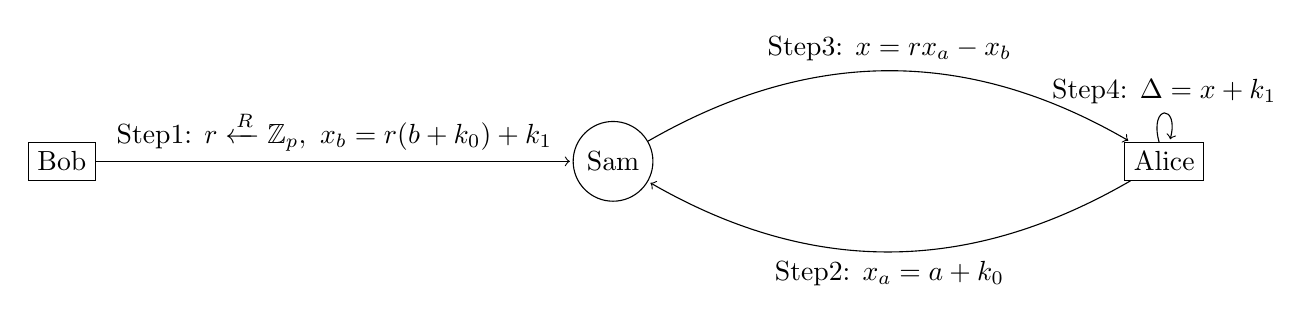
\begin{tikzpicture}[shorten >=1pt,node distance=7cm,on grid,auto]
            \node[draw,rectangle] (b) {Bob};
            \node[draw,circle] (s) [right=of b] {Sam};
            \node[draw,rectangle] (a) [right=of s] {Alice};
            \path[->]
            (b)
              edge node {Step1: \(r\xleftarrow{R}\mathbb Z_p,\ x_b=r(b+k_0)+k_1\)} (s)
            (a)
              edge [bend left] node {Step2: $x_a=a+k_0$} (s)
              edge [loop above] node {Step4: $\Delta=x+k_1$} (a)
            (s)
              edge [bend right=-30] node {Step3: $x=rx_a-x_b$} (a);           
        \end{tikzpicture}
        \caption{The protocol procedure}
        \label{fig:1}
    \end{figure}
    \\
    As $\Delta=x+k_1=r(a-b)$ so we get the condition that $r\neq0$
    \\
    if $(k_0,k_1)$ are used for more than once. 
    We assume it was tested if $a=b$ and $a^\prime=b^\prime$\\
    For Sam:
    \[
      \begin{cases}
        x_a=a+k_0\\
        x_b=r(b+k_0)+k_1
      \end{cases}
    \]
    \[
      \begin{cases}
        x_a^\prime=a^\prime+k_0\\
        x_b^\prime=r^\prime(b^\prime+k_0)+k_1
      \end{cases}
    \]
    So Sam learned that $a^\prime-a=x_a^\prime-x_a$. \\
    For Alice:
    \[
      \begin{cases}
        x=r(a-b)-k_1\\
        x^\prime=r^\prime(a^\prime-b^\prime)-k_1
      \end{cases}
    \]
    Alice learned ration of $(a-b)/(a^\prime-b^\prime)$ which reveal $b/b^\prime$\\

    \textbf{Bugfix}\\
    the core of the issue was the reusing of the $(k_0,k_1)$, so we should generate new indenpendent key from it by PRF. We define a secure PRF F defined at $\{K, \mathbb Z_b,\mathbb Z_p^2\}$ 
    we can derive the key-pair $(k_p,k_q)$ from $F$ and initial seed key $k$ as:
    $F(k, n)=(k_p,k_q)$ and $n$ is value of counter.\\
    We should let Alice and Bob get the value of counter synchronically for the syncronicity of key-pair. each time Alice and Bob finish the comparison, they increase the their counter by 1. 
    so they get the syncronical key-pair.
    \begin{figure}[h]
        \centering
        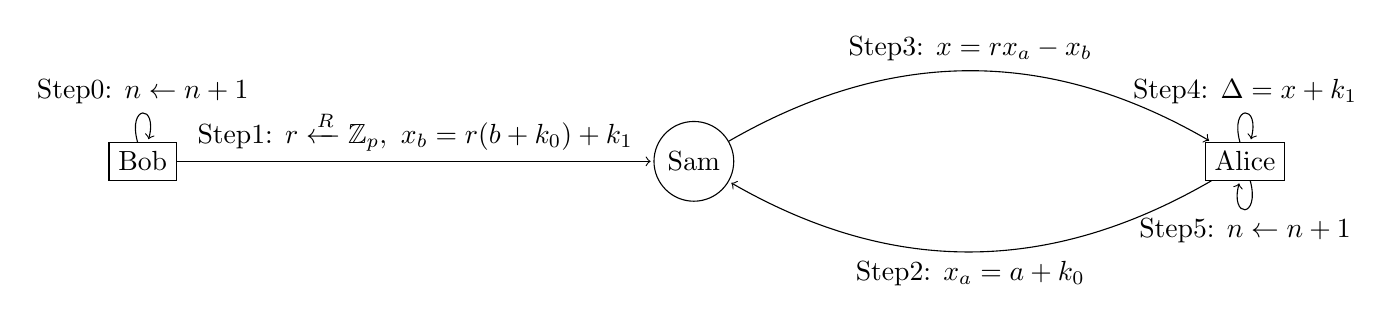
\begin{tikzpicture}[shorten >=1pt,node distance=7cm,on grid,auto]
            \node[draw,rectangle] (b) {Bob};
            \node[draw,circle] (s) [right=of b] {Sam};
            \node[draw,rectangle] (a) [right=of s] {Alice};
            \path[->]
            (b)
              edge node {Step1: \(r\xleftarrow{R}\mathbb Z_p,\ x_b=r(b+k_0)+k_1\)} (s)
              edge [loop above] node {Step0: $n\leftarrow n+1$} (a)
            (a)
              edge [bend left] node {Step2: $x_a=a+k_0$} (s)
              edge [loop above] node {Step4: $\Delta=x+k_1$} (a)
              edge [loop below] node {Step5: $n\leftarrow n+1$} (a)
            (s)
              edge [bend right=-30] node {Step3: $x=rx_a-x_b$} (a);           
        \end{tikzpicture}
        \caption{The fixed protocol procedure}
        \label{fig:2}
    \end{figure}
    
\end{homeworkProblem}
\end{document}
